\documentclass{article}

\usepackage[margin=1in]{geometry}
\usepackage{graphicx}

\title{Requirements specification for a Crux graphical user interface}

\author{William Stafford Noble\\
Department of Genome Sciences\\
Department of Computer Science and Engineering\\
University of Washington}

\begin{document}

\maketitle

\section{Introduction}

Crux is a software toolkit for analyzing shotgun proteomics data.
Currently, users apply these tools via a command line interace defined
with respect to a single binary executable.  The toolkit includes
tools for searching a sequence database, assigning statistical
confidence estimates to the resulting peptide-spectrum matches, and
inferring protein identifications from a collection of spectra.

We would like to provide a graphical user interface (GUI) that is
intuitive, flexible and portable.  Logistically, we have the following
design goals:
\begin{itemize}
\item Crux should run under Linux, MacOS and Windows.
\item Crux should be easy to install.
\item Any code that we use must be compatible with the Crux license.
\end{itemize}
More philosophical goals include the following:
\begin{itemize}
\item The Crux GUI should provide an easy way for a novice user to
  carry out common tasks, as well as flexibility for advanced users to
  perform more esoteric tasks.
\item For a multi-step analysis, a mechanism should be provided to
  allow the user to easily re-use steps from previous analyses.
\item Crux will not provide the functionality of a full laboratory
  information management system.
\end{itemize}

\section{A simple analysis}

\begin{figure}
\centering
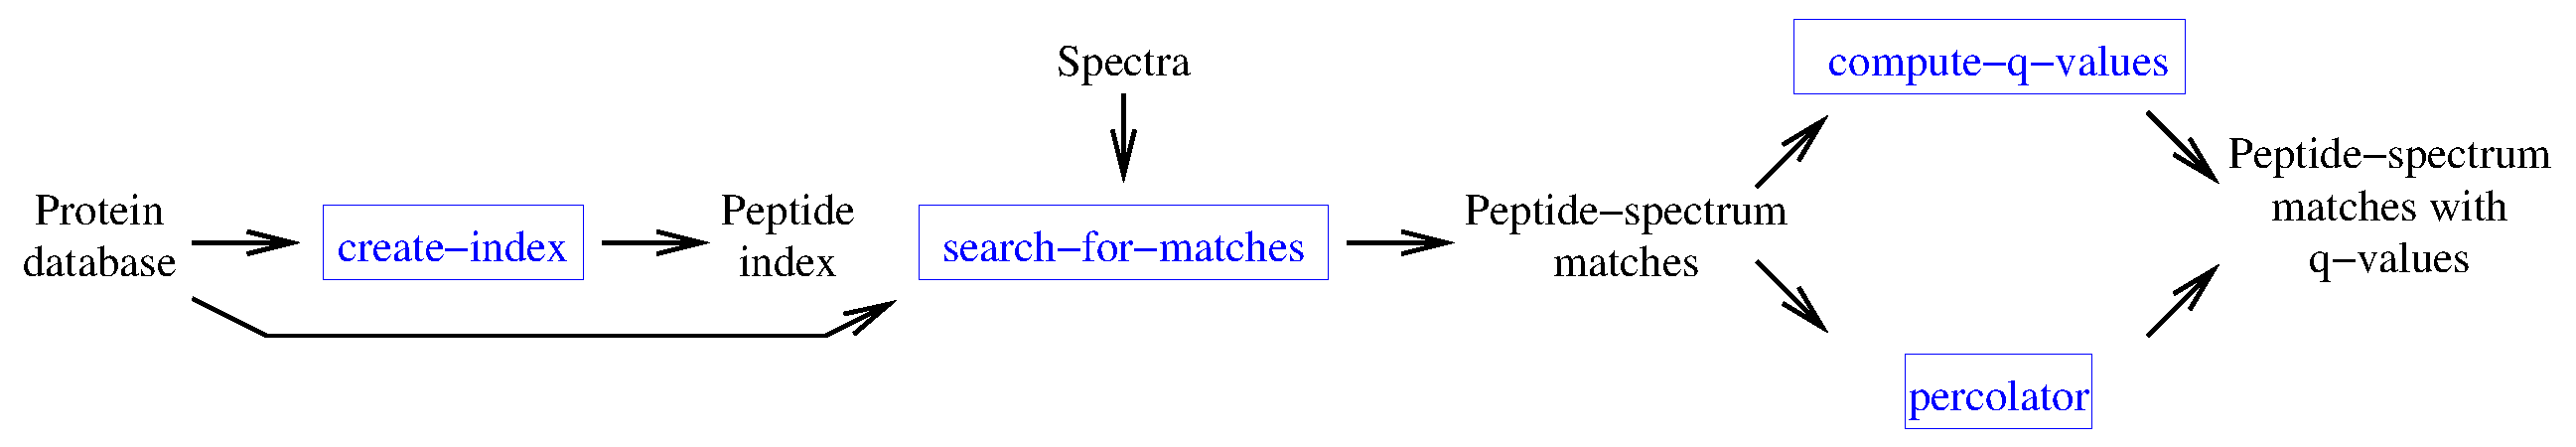
\includegraphics[width=6in]{schematic.eps}
\caption{{\bf The Crux toolkit.}  The figure shows the input/output
  relationships among the current set of tools in the Crux toolkit.
  \label{figure:schematic}}
\end{figure}

The first time a user runs Crux, they see a flow diagram showing the
input/output relationships among the various Crux tools, as in
Figure~\ref{figure:schematic}.  The user is asked to click on the
tools that they would like to use.  Clicking on a tool ``lights it
up'' in some fashion.  After lighting up one tool, clicking on a
mutually exclusive tool (i.e., clicking first percolator and then
compute-q-values) causes the first tool to go dark again.  Clicking on
a tool a second time also causes it to go dark.

When a tool is selected, input boxes for the required input files and
for several key parameters are displayed prominently, directly below
the schematic.  Optionally, the user can click on a ``Show additional
parameters'' button to display the complete list of parameters, with
their default values specified.

In addition to tool-specific parameters, Crux provides an option to
specify a name for this particular analysis.  Specifying such a name
will make it easier to retrieve the results of this analysis later.
If the user does not specify a name, then a name is created
automatically, using e.g., the name of the MS2 file and the date.

Once the user specifies, at the least, the inputs for the search
routine, the analysis can begin.  A ``Start analysis'' button appears
on the screen.  The user can continue modifying parameters as long as
they want, but they are free to start the analysis at any time.  At
that point, the analysis will begin, and the user is directed to an
output page.

The final output of the analysis is an XML ``summary file'' containing
links to the various tool outputs.  Initially, the summary file is
just a skeleton showing where the results will eventually appear, with
each tool listed as a link.  Links become live as soon as a tool
starts running, and the user can click on the link to see the current
progress of the job, or the final results.  Internally, each tool
creates its own directory, storing necessary parameters therein.  The
file simply links to these directories.  The file can be accessed via
a browser to view the results of the analysis, or the file can be
provided as input to Crux to initialize a subsequent analysis.

\section{Modifying a previous analysis}

To re-run an analysis, the user starts Crux and provides as input the
summary file produced by the previous analysis.  The Crux flow diagram
is displayed again, and boxes corresponding to analyses that have
already been run are indicated visually in some way.  Thus, in
general, each box takes one of three states: unselected, selected but
not run yet, or complete.

Most commonly, a user will want to re-run the same analysis on new
spectra.  In this case, they click on the ``search-for-matches'' box
and enter the name of a new MS2 file.  At this point, that box
switches to the ``not run yet'' state, and all of the downstream boxes
do as well.  Selected parameter settings remain the same.

Prior to re-running the analysis, the user must select a new name for
the experiment.  If they do not do so, then they will be asked whether
it is OK to delete the results of the previous analysis.  If the user
says ``yes,'' then the directories associated with the modified
analysis steps are deleted prior to starting the analysis.  If the
user says ``no,'' then the user is given the option of providing a new
name for the experiment.

\section{Robustness}

Crux assumes that the user will not disrupt the directory structure
that the toolkit creates.  The structure itself is quite simple: each
analysis consist of one summary file, plus a set of linked
directories, one per tool.  It is OK for a user to delete or move one
of these directories, but if they try to run Crux using the summary
file, the tool corresponding to the missing directory will be
indicated as ``not run yet,'' as will all downstream tools.
Similarly, if the user moves the summary file without moving the
corresponding tool-specific directories, then when Crux is run using
that summary file, all of the analyses will be displayed as ``not run
yet.''  Note that, since the parameters are all stored in the relevant
subdirectories, deleting or moving a tool-specific subdirectory will
result in re-setting all the parameters to their default values.

In general, the name that the user provides will be the name of the
summary file (with .xml appended).  Thus, re-running the same analysis
multiple times requires clobbering the corresponding output file and
output directories.  The GUI maintains internal logic indicating the
status of each job (not-run-yet, to-be-run, unselected).  Prior to any
analysis, the GUI checks whether any of the to-be-run jobs already
have output directories associated with them.  In this case, the user
is queried, as described above, whether to delete the problematic
directories or re-name the analysis.

Power users might want to cobble together different analyses, by
selecting output directories from different tools and creating their
own summary script.  They do so at their own risk.  In such a
scenario, the settings from one directory may not be compatible with
the settings in a downstream directory.

\section{A common single-tool interface}

The Crux summary page created by a single analysis contains links to
output directories created by each tool.  Clicking on any of these
links leads to a tool-specific summary page.  All tools create summary
pages that share a common ``look and feel.''  Each such page contains
a brief summary of the analysis, with links to a parameter file,
a log file, the input files and each of the output files.

The indexing tool does not create user-level output files.  Instead,
the summary page simply lists some basic statistics about the index:
the total number of proteins in the index, the average protein length,
the total number of peptides in the index, the average number of
peptides per protein, the average peptide length.

\section{Manipulating ranked lists}

Most Crux tools create, as their primary output, a ranked list of
objects---PSMs, peptides or proteins.  Eventually, we would like to
create an interface that allows users to maniuplate these ranked lists
in the following ways:
\begin{itemize}
\item Features (columns) can be hidden or displayed, at the user's
  discretion.
\item The list can be sorted according to the values in one or more
  columns, in either ascending or descending order.
\item The list can be thresholded according to the values in one or
  more columns, using either a maximum or minimum value.
\item A protein-level ranking can be expanded (either globally or on a
  per-protein basis) to list peptides, and peptides can in turn be
  expanded to list individual spectra.
\item Spectra can optionally be expanded to display clickable
  thumbnail images, with various types of peaks (b- and y-ions)
  annotated in color.
\end{itemize}
Because creating such an interface promises to be onerous, this
activity will be shelved for the foreseeable future.

\end{document}
